%!TEX root = /Users/nunolourenco/Documents/FCTUC/Mestrado/2010_2011/Thesis/Thesis/thesis.tex
\chapter{Results}
\label{chap:results}

In this chapter we present an experimental analysis of the application of our algorithm to several instances of short-ranged Morse Clusters. To perform such analysis, we start by describing the scenario used in our experiments. In Section \ref{sec:experimental_results} we present and discuss the results obtained by the DACCO algorithm. In Section \ref{sec:algorithm_comparison} we present a comparative analysis between DACCO and other approaches of the literature. Finally, in Section \ref{sec:detailed_analysis} we present a detailed analysis of some main components of the algorithm.

\section{Experimental Scenario}
\label{sec:experimental_scenario}
In this study we focus our attention in several instances of short-ranged Morse clusters. More precisely, we selected instances with a number of atoms that ranges between 30 and 50. With this scenario we aim for two goals: 
	\begin{enumerate}
		\item Assess the performance of the algorithm;
		\item Gain insight into the influence of some components of the algorithm. 
	\end{enumerate}
	For the first objective, we present the results of the DACCO optimization for all the aforementioned instances, and we analyze its performance based on two criteria:
	\begin{enumerate}
		\item Ability to discover the known optima;
		\item Mean Best Fitness (MBF) and deviation from the optimum;
	\end{enumerate}
	The first criterion is a widely adopted performance measure in cluster geometry optimization. Hence, for all instances, we show its success rate(number of times that it found the best-known solution) of the algorithm. In case it does not find the best-known solution we present the best solution found by the algorithm. The second criterion aims to complement our study, as it will provide information about the ability of DACCO to converge to promising areas of the search space.\\
	Later, to assess the absolute performance of the DACCO, we compare its results with those achieved by two algorithms: a steady-state EA described in Pereira et al. \cite{xico09}, and the Particle Swarm Optimization algorithm (PSO) described in Lourenço et al. \cite{lourenco11}.
\section*{Experimental Settings} \label{sec:experimental_setting}
\begin{table}[t]
	\begin{center}
		\begin{tabular}{| l | p{8cm} |}
			\hline
			\textbf{Parameter} & \textbf{Value} \\ \hline
			Runs & 30 \\
			Population size & Equal to the number of atoms $N$\\
			Number of evaluations & 5000000 \\
			Morse Potential range $(\beta)$ & 14.0 \\ 
			Cell size $(W)$ & 0.6 \\
			Number of Atoms $(N)$ & Between 30 and 50 \\
			Influence of the pheromones $(\alpha)$ & 4 \\
			Continuous Local Search Iterations & 1000\\
			Continuous Local Search Accuracy & 1.0E-8\\
			Pheromone propagation value ($p$) & 0.5 \\
			Neighborhood type & Moore Neighborhood \\
			Neighborhood radius $(r)$ & 3 \\
			Discrete Local Search Iteration & 10 \\
			\hline
		\end{tabular}
	\caption{Parameter setting used in the experiments}
	\label{tab:general_settings}
	\end{center}
\end{table}
Table \ref{tab:general_settings} lists the general parameters used in all of the experiments. We performed a total of 30 runs to make possible a statistical analysis. In each run we allowed our algorithm to perform 5000000 evaluations. It is important to refer that each iteration made by L-BFGS procedure counts as one evaluation. 
The size of the population depends on the size of the cluster being optimized. This parameter was set based on the reviewed literature, and some preliminary tests. The cell size ($W$) corresponds to size of each cell in our search space. The neighborhood used is the Moore neighborhood with $r = 3$. The number of iterations in the discrete local search is 10. The $\alpha$ value was set to 4, following the reviewed literature, and after the analysis of some preliminary results.

\section*{Statistical Analysis}
\label{sec:statistical_analysis}
While comparing our algorithm with the EA and the PSO we performed a statistical analysis to validate the results. We assumed that our data did not followed any distribution. Thus we applied the Mann-Whitney non-parametric test, at a 0.05 level of significance, to assess the statistical differences of the means, over the 30 runs of each of pair DACCO-EA and DACCO-PSO of algorithms. Furthermore the same test is used to perform a detailed analysis in the components of the algorithm. For multiple comparisons the $p$-value (0.05) used was adjusted using the Bonferroni correction method. To perform such correction we used used the following equation:
\begin{equation}
	p_B = \frac{p} {nc}
\end{equation}

where $nc$ is the number of comparisons performed, and the $p_B$ is the $p$-value to consider.

The hypothesis for comparing two algorithms were:
\begin{itemize}
	\item $H_{0} : u_1 = u_2$ - means of the algorithms were equal, as the null hypothesis.
	\item $H_{1} : u_1 \neq u_2$ - means of the algorithms were not equal, as the alternative hypothesis.
\end{itemize}

Each time we applied a statistical test we looked for the results and concluded: if the $p$-value of the statistical test was smaller than the level of confidence, there was evidence to reject the null hypothesis $H_{0}$, and we could accept the alternative $H_{1}$. This means that there was evidence that the means were significantly different  at the significance level of 0.05. In contrast, there was not enough evidence to reject $H_{0}$, and being so, we concluded that the means were not significantly different.

In the tables where we make the statistical analysis we use the following notation: ``>" when the means are statistical different, and the first algorithm presents an higher mean value than the second, ``<"  when the means are statistical different, and the second algorithm presents an higher mean value than the first, and ``$\sim$" when there is no statistical differences in the means.



\section{DACCO: Experimental Results}
\label{sec:experimental_results}
	
	In Table \ref{tab:optimization_results} we present the optimization results of short-ranged Morse Clusters between 30 and 50 obtained by the DACCO algorithm. The first column, \emph{Instance}, identifies the number of atoms of each cluster. The second column, \emph{Optimum}, displays the potential energy of the best-known solution. The third column, \emph{Best Solution Found}, displays the potential energy of the best solution found by the DACCO. The next two columns present the success rate (column \emph{SR}) and the Mean Best Fitness (column \emph{MBF}). The last column measures of how the MBF deviates, in percentage, from the best-known solution.
	\begin{table}[!htbp]
		\begin{center}
			\begin{tabular}{| c | c | p{3cm} | c | c | p{2cm} |}
				\hline
				\textbf{Instance} & \textbf{Optimum} & \textbf{Best Solution Found} & \textbf{SR} & \textbf{MBF} & \textbf{Deviation}\\ \hline
				30 & -106.835790 & -106.835790 & 28 / 30 & -106.831095 & 0.004 \\ \hline
				31 & -111.760670 & -111.760670 & 30 / 30 & -111.760670 & 0.000 \\ \hline
				32 & -115.767561 & -115.767561 & 30 / 30 & -115.767561 & 0.000 \\ \hline
				33 & -120.741345 & -120.741345 & 30 / 30 & -120.741345 & 0.000 \\ \hline
				34 & -124.748271 & -124.748271 & 30 / 30 & -124.748271 & 0.000 \\ \hline
				35 & -129.737360 & -129.737360 & 30 / 30 & -129.737360 & 0.000 \\ \hline
				36 & -133.744666 & -133.744666 & 30 / 30 & -133.744666 & 0.000 \\ \hline
				37 & -138.708582 & -138.708582 & 28 / 30 & -138.682731 & 0.019 \\ \hline
				38 & -144.321054 & -144.321054 & 25 / 30 & -144.053535 & 0.185 \\ \hline
				39 & -148.327400 & -148.327400 & 26 / 30 & -148.243303 & 0.057 \\ \hline
				40 & -152.333745 & -152.333745 & 25 / 30 & -152.228797 & 0.069 \\ \hline
				41 & -156.633479 & -156.633479 & 11 / 30 & -156.483040 & 0.096 \\ \hline
				42 & -160.641020 & -160.641020 & 5 / 30 & -160.449243 & 0.119 \\ \hline
				43 & -165.634973 & -165.634973 & 6 / 30 & -165.361457 & 0.165 \\ \hline
				44 & -169.642441 & -169.642441 & 3 / 30 & -169.383463 & 0.153 \\ \hline
				45 & -174.511632 & -174.511632 & 3 / 30 & -174.295931 & 0.124 \\ \hline
				46 & -178.519320 & -178.519320 & 2 / 30 & -178.371855 & 0.083 \\ \hline
				47 & -183.508227 & -183.411312 & 0 / 30 & -183.095976 & 0.225 \\ \hline
				48 & -188.888965 & -188.888965 & 19 / 30 & -188.402414 & 0.258 \\ \hline
				49 & -192.898412 & -192.898412 & 15 / 30 & -192.675230 & 0.116 \\ \hline
				50 & -198.455632 & -198.455632 & 12 / 30 & -197.853115 & 0.304 \\ \hline
			\end{tabular}
		\caption{Optimization results of Morse Clusters between 30 and 50 obtained by DACCO}
		\label{tab:optimization_results}
		\end{center}
	\end{table}
	
	The results from Table \ref{tab:optimization_results} are encouraging, since the proposed approach was able to find almost all the best-known solutions for short-ranged Morse clusters between 30 and 50, missing only 1 instance.
	To the best of our knowledge, this is the first work to apply ACO algorithm to the problem of cluster geometry optimization, hence its results may play an important role in future proposals that intend to use the same approach.
	
	By analyzing the success rate of the algorithm we noticed that its variation is irregular: whereas between 30 and 40 atoms the success rate is high, for clusters between 41 and 50 atoms the algorithm has more difficulties to find the optimum. This can in part be explained, by the fact the we keep the number of evaluation fixed for all the clusters. With more atoms, we will get a larger search space, and it is not surprising that the performance of the algorithm declines.
	
	Looking at the MBF values, they are always close to the optimum, as the deviation values range between 0.000 \% and 0.304 \%. This result is interesting, as it shows that even if DACCO converges to local optima, it can accurately find low potential structures.
	
	Another interesting aspect is that DACCO has a good performance while optimizing the so called ``magic instances" of 30 and 38 atoms \cite{doye97}. These instances define particularly rugged landscapes, and the majority of the unbiased algorithms tend to converge to local optima \cite{doye97, grosso07}.
	
	\section{Algorithm Comparison}
	\label{sec:algorithm_comparison}
	In this section we compare our approach with others described in the literature. A direct comparison with other ACO approaches its not possible, due to absence of such approaches. Hence, we compare our approach with one of the Swarm Intelligence algorithms family, and with an another of the Evolutionary Algorithms family.
	
	\subsection{DACCO versus PSO}
	In Table \ref{tab:dacco_vs_pso} we compare the DACCO and PSO algorithms. The third and fourth column represent the success rate (SR) and the MBF of DACCO. The last two columns represent the SR and the the MBF of PSO. 
	
	The number of evaluations granted to the PSO algorithm were the same of the DACCO. 
	
	\begin{table}[!htdp]
			\begin{center}
				\begin{tabular}{| c | c | c | c | c | c |}
					\hline
					\multicolumn{2}{|c|}{} & \multicolumn{2}{c|}{\textbf{DACCO}} & \multicolumn{2}{c|}{\textbf{PSO}}\\ \hline
					\textbf{Instance} & \textbf{Optimum} & \textbf{SR} & \textbf{MBF} & \textbf{SR} & \textbf{MBF} \\ \hline
					30 & -106.835790 & 28 / 30 & -106.831095 & 4 / 30 & -106.718221 \\ \hline
					31 & -111.760670 & 30 / 30 & -111.760670 & 19 / 30 & -111.630904 \\ \hline
					32 & -115.767561 & 30 / 30 & -115.767561 & 20 / 30 & -115.686360 \\ \hline
					33 & -120.741345 & 30 / 30 & -120.741345 & 19 / 30 & -120.690258 \\ \hline
					34 & -124.748271 & 30 / 30 & -124.748271 & 15 / 30 & -124.605299 \\ \hline
					35 & -129.737360 & 30 / 30 & -129.737360 & 6 / 30 & -129.078905 \\ \hline
					36 & -133.744666 & 30 / 30 & -133.744666 & 14 / 30 & -133.494812 \\ \hline
					37 & -138.708582 & 28 / 30 & -138.682731 & 12 / 30 & -138.147442 \\ \hline
					38 & -144.321054 & 25 / 30 & -144.053535 & 8 / 30 & -142.545537 \\ \hline
					39 & -148.327400 & 26 / 30 & -148.243303 & 7 / 30 & -147.361971 \\ \hline
					40 & -152.333745 & 25 / 30 & -152.228797 & 7 / 30 & -151.516586 \\ \hline
					41 & -156.633479 & 11 / 30 & -156.483040 & 2 / 30 & -155.898689 \\ \hline
					42 & -160.641020 & 5 / 30 & -160.449243 & 4 / 30 & -160.027062 \\ \hline
					43 & -165.634973 & 6 / 30 & -165.361457 & 4 / 30 & -164.649840 \\ \hline
					44 & -169.642441 & 3 / 30 & -169.383463 & 3/ 30 & -168.908517 \\ \hline
					45 & -174.511632 & 3 / 30 & -174.295931 & 3 / 30 & -173.160552 \\ \hline
					46 & -178.519320 & 2 / 30 & -178.371855 & 1 / 30 & -177.513539 \\ \hline
					47 & -183.508227 & 0 / 30 & -183.095976 & 1 / 30 & -182.081130 \\ \hline
					48 & -188.888965 & 19 / 30 & -188.402414 & 2 / 30 & -186.782038 \\ \hline
					49 & -192.898412 & 15 / 30 & -192.675230 & 4 / 30 & -191.496032 \\ \hline
					50 & -198.455632 & 12 / 30 & -197.853115 & 1 / 30 & -195.816027 \\ \hline
				\end{tabular}
			\end{center}
			\caption{Experimental results of Morse cluster between 30 and 50 atoms obtained by the DACCO algorithm and the PSO}
			\label{tab:dacco_vs_pso}
		\end{table}
		
		Looking at the results, we can conclude that the DACCO is better than PSO. We can see that, for almost all instances the SR of DACCO is higher than the SR of the PSO. It misses only the 47 atoms instance. Furthermore, analyzing the MBF values the DACCO presents the better values for all instances. These MBF results are interesting because they show that the DACCO algorithm can find solutions with better quality than the ones of the PSO. To confirm this, in Fig. \ref{fig:dacco_pso_mbf_50} we present the evolution of the MBF for DACCO and PSO. The results are from the Morse cluster with 50 atoms, but the same trend is visible for other instances. The information in the chart shows that the MBF of the DACCO is lower during the whole optimization process.
		\botapic[0.5]{dacco_pso_mbf_50}{Evolution of the MBF of DACCO and PSO. The results were obtained with the Morse cluster of 50 atoms.}
		\begin{table}[!htdp]
				\begin{center}
					\begin{tabular}{| c | c |}
						\hline
						\textbf{Instance} & \textbf{DACCO-PSO} \\ \hline
						30 & > \\ \hline
						31 & > \\ \hline
						32 & > \\ \hline
						33 & > \\ \hline
						34 & > \\ \hline
						35 & > \\ \hline
						36 & > \\ \hline
						37 & > \\ \hline
						38 & > \\ \hline
						39 & > \\ \hline
						40 & > \\ \hline
						41 & > \\ \hline
						42 & > \\ \hline
						43 & > \\ \hline
						44 & > \\ \hline
						45 & > \\ \hline
						46 & > \\ \hline
						47 & > \\ \hline
						48 & > \\ \hline 
						49 & > \\ \hline
						50 & > \\ \hline
					\end{tabular}
					\caption{Statistical results of comparing DACCO and PSO}
					\label{tab:statistical_comparison_pso}
				\end{center}
		\end{table}
		\\ Looking at Table \ref{tab:statistical_comparison_pso}, we can see that the means of DACCO are statistical different and they have an higher value. Hence we can concluded that DACCO performs better than the PSO.
		\pagebreak
		\subsection{DACCO versus EA}
		
			In Table \ref{tab:dacco_vs_ea} we compare the DACCO and EA algorithms. Like in the previous section, the third and fourth column represent SR and the MBF of DACCO. The last two columns represent the SR and the the MBF of EA. Again, the number of evaluation granted to the EA, was the same of the DACCO. 
		\begin{table}[!htdp]
				\begin{center}
					\begin{tabular}{| c | c | c | c | c | c |}
						\hline
						\multicolumn{2}{|c|}{} & \multicolumn{2}{c|}{\textbf{DACCO}} & \multicolumn{2}{c|}{\textbf{EA}}\\ \hline
						\textbf{Instance} & \textbf{Optimum} & \textbf{SR} & \textbf{MBF} & \textbf{SR} & \textbf{MBF} \\ \hline
						30 & -106.835790 & 28 / 30 & -106.831095 & 22 / 30 & -106.794747 \\ \hline
						31 & -111.760670 & 30 / 30 & -111.760670 & 30 / 30 & -111.760670 \\ \hline
						32 & -115.767561 & 30 / 30 & -115.767561 & 29 / 30 & -115.766686 \\ \hline
						33 & -120.741345 & 30 / 30 & -120.741345 & 28 / 30 & -120.697611 \\ \hline
						34 & -124.748271 & 30 / 30 & -124.748271 & 28 / 30 & -124.715475 \\ \hline
						35 & -129.737360 & 30 / 30 & -129.737360 & 27 / 30 & -129.623232 \\ \hline
						36 & -133.744666 & 30 / 30 & -133.744666 & 28 / 30 & -133.715154 \\ \hline
						37 & -138.708582 & 28 / 30 & -138.682731 & 25 / 30 & -138.610585 \\ \hline
						38 & -144.321054 & 25 / 30 & -144.053535 & 8 / 30 & -143.130422 \\ \hline
						39 & -148.327400 & 26 / 30 & -148.243303 & 14 / 30 & -147.958055 \\ \hline
						40 & -152.333745 & 25 / 30 & -152.228797 & 9 / 30 & -151.886095 \\ \hline
						41 & -156.633479 & 11 / 30 & -156.483040 & 15 / 30 & -156.547928 \\ \hline
						42 & -160.641020 & 5 / 30 & -160.449243 & 12 / 30 & -160.518149 \\ \hline
						43 & -165.634973 & 6 / 30 & -165.361457 & 14 / 30 & -165.254805 \\ \hline
						44 & -169.642441 & 3 / 30 & -169.383463 & 7 / 30 & -169.303639 \\ \hline
						45 & -174.511632 & 3 / 30 & -174.295931 & 5 / 30 & -174.102119 \\ \hline
						46 & -178.519320 & 2 / 30 & -178.371855 & 9 / 30 & -178.389713 \\ \hline
						47 & -183.508227 & 0 / 30 & -183.095976 & 2 / 30 & -183.153610 \\ \hline
						48 & -188.888965 & 19 / 30 & -188.402414 & 14 / 30 & -188.160694 \\ \hline
						49 & -192.898412 & 15 / 30 & -192.675230 & 18 / 30 & -192.627890 \\ \hline
						50 & -198.455632 & 12 / 30 & -197.853115 & 5 / 30 & -197.688978 \\ \hline
					\end{tabular}
				\end{center}
				\caption{Experimental results of Morse cluster between 30 and 50 atoms obtained by the DACCO algorithm and the EA}
				\label{tab:dacco_vs_ea}
			\end{table}
			An overview of the results presented in Table \ref{tab:dacco_vs_ea} reveal that DACCO has as good results as those of EA for the considered Morse clusters. Moreover, looking at the MBF values of both algorithms, we can see that they are very close, revealing that the solutions found by DACCO are as good as the ones found by the EA. To confirm this, in Fig. \ref{fig:dacco_ea_mbf_50} we present the evolution of the MBF for DACCO and the EA. The results are from the Morse cluster with 50 atoms, but the same trend is visible for other instances. By observing it we see that the MBF of DACCO tends to converge more rapidly than the MBF of the EA. However, at the end of the optimization process the MBF of DACCO and of EA tend to get equal.\\
			Table \ref{tab:statistical_comparison_ea} shows that DACCO is as effective as the EA.
			\begin{table}[!htdp]
					\begin{center}
						\begin{tabular}{| c | c |}
							\hline
							\textbf{Instance} & \textbf{DACCO-EA} \\ \hline
							30 & > \\ \hline
							31 & $\sim$ \\ \hline
							32 & $\sim$ \\ \hline
							33 & $\sim$ \\ \hline
							34 & $\sim$ \\ \hline
							35 & $\sim$ \\ \hline
							36 & $\sim$ \\ \hline
							37 & $\sim$ \\ \hline
							38 & > \\ \hline
							39 & > \\ \hline
							40 & > \\ \hline
							41 & $\sim$ \\ \hline
							42 & $\sim$ \\ \hline
							43 & $\sim$ \\ \hline
							44 & $\sim$ \\ \hline
							45 & $\sim$ \\ \hline
							46 & $\sim$ \\ \hline
							47 & $\sim$ \\ \hline
							48 & $\sim$ \\ \hline 
							49 & $\sim$ \\ \hline
							50 & $\sim$ \\ \hline
						\end{tabular}
						\caption{Statistical results of comparing DACCO and EA}
						\label{tab:statistical_comparison_ea}
					\end{center}
			\end{table}
			\botapic[0.45]{dacco_ea_mbf_50}{Evolution of the MBF of DACCO and EA. The results were obtained with the Morse cluster of 50 atoms.}
		
		It is important to note that in four Morse instances our approach has statistical differences in the means. Some of these Morse instances,  the ones with 30 and 38 atoms, are particularly hard to optimize, as they define very roughed landscapes, with many local minima \cite{doye97}.\\
		
		Moreover, these results show that DACCO can compete with the EA, while optimizing Morse clusters with a number of atoms between 30 and 50. This is an important outcome since the EA used for comparison is a state-of-art method, and the algorithm proposed in this dissertation performs as good as it.


		\section{Detailed Analysis}
		\label{sec:detailed_analysis}
		
		DACCO contains some components that enhance its effectiveness in cluster geometry optimization problems. In this section we present a set of additional tests to clarify the importance of some of these components. We selected clusters with size $N=\{30, 38, 45, 50\}$, and changes range from simple parameter setting variation to structural modifications in the DACCO framework. All comparisons in this work are made between the final DACCO version. These comparisons of results will help to clarify the influence of the different components used.
		
		
		\subsection{Cell Size}
		In this section we present the results of the variation of the cell size $W$. When we have a big $W$ our search space will be smaller, but we will start to have more than on atom in one cell. Furthermore we have to be careful while defining the cell size, because we need to guarantee that our cube can host an entire cluster. Taking this into account it is important to assess how the algorithm behaves with different cell sizes.
		Table \ref{tab:cell_size_results} present results obtained with additional setting $W=\{0.5, 0.6, 0.7\}$. A inspection of this table reveals that the outcomes of the optimization, with different $W$ are similar.
		There is a slight trend for the $W=0.6$ to obtain results of higher quality in both terms of success rate and MBF (Fig. \ref{fig:mbf_cell_size_50}).
		We performed a statistical analysis to confirm that there is no statistical evidence to which one of the $W$ values is better.
		   		
		\begin{table}[!htdp]
				\begin{center}
					\begin{tabular}{| c | c | c | c | c | c | c |}
						\hline
						\textbf{Instance} & \multicolumn{2}{c|}{\textbf{$W=0.5$}} & \multicolumn{2}{c|}{\textbf{$W=0.6$}} & \multicolumn{2}{c|}{\textbf{$W=0.7$}} \\ \hline
						~ & SR & MBF & SR & MBF & SR & MBF \\ \hline
						30 & 28 / 30 & -106.831095 & 28 / 30 & -106.831095 & 30 / 30 & -106.835790 \\ \hline
						38 & 20 / 30 & -143.786016 & 25 / 30 & -144.053535 & 19 / 30 & -143.732512 \\ \hline
						45 & 1 / 30 & -174.304756 & 3 / 30 & -174.295931 & 2 / 30 & -174.331536 \\ \hline
						50 & 4 / 30 & -197.694748 & 12 / 30 & -197.853115 & 9 / 30 & -197.831498 \\ \hline
					\end{tabular}
					\caption{Optimization results obtained by DACCO with different values of $W$ in the selected Morse cluster instances}
					\label{tab:cell_size_results}
				\end{center}
		\end{table}
		\botapic[0.45]{mbf_cell_size_50}{Evolution of the MBF of DACCO with different values of $W$. Results were obtained with the Morse instance with 50 atoms.}
		
		
		
		% \begin{table}[!htdp]
		% 				\begin{center}
		% 					\begin{tabular}{| c | c | c | c |}
		% 						\hline
		% 						\textbf{Instance} & \textbf{$W=0.5$ - $W=0.6$} & \textbf{$W=0.5$ - $W=0.7$} & \textbf{$W=0.6$ - $W=0.7$} \\ \hline
		% 						30 & $\sim$ & $\sim$ & $\sim$ \\ \hline
		% 						38 & $\sim$ & $\sim$ & $\sim$ \\ \hline
		% 						45 & $\sim$ & $\sim$ & $\sim$ \\ \hline
		% 						50 & $\sim$ & $\sim$ & $\sim$ \\ \hline
		% 					\end{tabular}
		% 					\caption{Statistical results of comparing the different cell sizes}
		% 					\label{tab:statistical_comparison_cell_size}
		% 				\end{center}
		% 		\end{table}
		
		
		
		\subsection{Neighborhoods}
		In this section we compare two neighborhoods: the Moore Neighborhood and the Full Moore Neighborhood. We used the same $r = 3$ for both neighborhoods.
		
		Table \ref{tab:neighborhood_results} present the results for both neighborhoods. Looking to the outcomes, we can see that for small instances the two neighborhoods have similar results. However, looking for the results obtained in larger instances, the Moore Neighborhood has better results. This may be explained by the fact that in the Full Moore neighborhood we are taking into account much more cells, and thus, the cell selection process can become to greedy. \\
		Table \ref{tab:statistical_comparison_neighborhoods} shows that for the bigger instances, the algorithm using the Moore neighborhood has statistical differences in the means when compared to the Full Moore neighborhood. Fig. \ref{fig:neighborhoods_mbf_50} presents the evolution of the MBF, and confirms that the Moore neighborhood achieves better results. 
		\begin{table}[!htdp]
				\begin{center}
					\begin{tabular}{| c | c | c | c | c |}
						\hline
						\textbf{Instance} & \multicolumn{2}{c|}{\textbf{Moore}} & \multicolumn{2}{c|}{\textbf{Full Moore}} \\ \hline
						~ & SR & MBF & SR & MBF \\ \hline
						30 & 28 / 30 & -106.831095 & 25 / 30 & -106.823627 \\ \hline
						38 & 25 / 30 & -144.053535 & 23 / 30 & -143.942889 \\ \hline
						45 & 3 / 30 & -174.295931 &  1 / 30 &  -173.998727 \\ \hline
						50 & 12 / 30 & -197.853115 & 3 / 30 &  -197.001784 \\ \hline
					\end{tabular}
					\caption{Optimization results obtained by DACCO with different Neighborhoods in the selected Morse cluster instances}
					\label{tab:neighborhood_results}
				\end{center}
		\end{table}
		\begin{table}[!htdp]
				\begin{center}
					\begin{tabular}{| c | c |}
						\hline
						\textbf{Instance} & \textbf{Moore - Full Moore} \\ \hline
						30 & $\sim$ \\ \hline
						38 & $\sim$ \\ \hline
						45 & > \\ \hline
						50 & > \\ \hline
					\end{tabular}
					\caption{Statistical results of comparing the different neighborhoods}
					\label{tab:statistical_comparison_neighborhoods}
				\end{center}
		\end{table}
		\botapic[0.45]{neighborhoods_mbf_50}{Evolution of the MBF of DACCO with different Neighborhoods. Results were obtained with the Morse instance with 50 atoms.}
		\pagebreak
		\subsection{Neighborhood Radius}
		
		In this section we compare the radius of the two neighborhoods. Using the Moore Neighborhood, we tried experimented values of $r = \{1, 2, 3, 4\}$ while optimizing the subset of instances.
		
		Table \ref{tab:neighborhood_radius_results} present the results of the optimization. Looking at the results, we can observe that choosing a small radius ($r=1$), the optimization process becomes too greedy, in a way that it always tries to build compact clusters. This works well for small instances, but for the large ones, we need some more freedom to place the atoms. However, with a large radius the optimization process starts to behave like the Full Moore Neighborhood. 
		
		Looking at these results, it is clear that we need to have a radius that is neither to small that it only looks at the closest positions, neither too large, that it starts destroying the cohesion of the cluster.
		
		In Table \ref{tab:statistical_comparison_radius} we present a statistical analysis of the radius used for experimentation. It clearly confirms that small radius do not help the search.
		
		Fig. \ref{fig:neighborhoods_radius_50} presents the evolution of the MBF for the different values of $r$. These figures confirms that, with low values of $r$, the algorithm converges to local optima of inferior quality when compared, for example, with $r=2$ or $r=3$. Moreover, this chart shows that with $r=4$ the MBF is smaller than the MBF of the version that uses $r=3$
		
		
		\botapic[0.50]{neighborhoods_radius_50}{Evolution of the MBF of DACCO with different values of $r$. Results were obtained with the Morse instance with 50 atoms.}
		
		
		\begin{landscape}
			 \begin{table}[!htdp]
					\begin{center}
						\begin{tabular}{| c | c | c | c | c | c | c | c | c |}
							\hline
							\textbf{Instance} & \multicolumn{2}{c|}{\textbf{r = 1}} & \multicolumn{2}{c|}{\textbf{r = 2}} & \multicolumn{2}{c|}{\textbf{r = 3}} & \multicolumn{2}{c|}{\textbf{r = 4}} \\ \hline
							~ & SR & MBF & SR & MBF & SR & MBF & SR & MBF \\ \hline
							30 & 22 / 30 & -106.816158 & 27 / 30 & -106.828748 & 28 / 30 & -106.831095 & 27 / 30 & -106.828748 \\ \hline
							38 & 28 / 30 & -144.211960 & 25 / 30 & -144.052332 & 25 / 30 & -144.053535 & 23 / 30 & -143.946527 \\ \hline
							45 & 0 / 30 & -173.593068 & 4 / 30 & -174.338129 & 3 / 30 & -174.295931& 1 / 30 & -174.338283 \\ \hline
							50 & 0 / 30 & -196.105401 & 7 / 30 & -197.387273 & 12 / 30 & -197.853115 & 4 / 30 & -197.605420 \\ \hline
						\end{tabular}
						\caption{Optimization results obtained by DACCO with different values of $r$ in the selected Morse cluster instances}
						\label{tab:neighborhood_radius_results}
					\end{center}
			\end{table}
		
			\begin{table}[!htdp]
					\begin{center}
						\begin{tabular}{| c | c | c | c | c | c | c |}
							\hline
							\textbf{Instance} & \textbf{r = 1 - r = 2} & \textbf{r = 1 - r = 3} & \textbf{r = 1 - r = 4} & \textbf{r = 2 - r = 3} & \textbf{r = 2 - r = 4} & \textbf{r = 3 - r = 4} \\ \hline
							30 & $\sim$ & $\sim$ & $\sim$ & $\sim$ & $\sim$ & $\sim$ \\ \hline
							38 & $\sim$ & $\sim$ & $\sim$ & $\sim$ & $\sim$ & $\sim$ \\ \hline
							45 & < & < & < & $\sim$ & $\sim$ & $\sim$ \\ \hline
							50 & < & < & < & $\sim$ & $\sim$ & $\sim$ \\ \hline
						\end{tabular}
						\caption{Statistical results of comparing the neighborhood radius}
						\label{tab:statistical_comparison_radius}
					\end{center}
			\end{table}
			
			\end{landscape}
			
		\subsection{Discrete Local Search}
		
		In this section we analyze the DACCO algorithm with and without the discrete local search procedure. 
		
		The discrete local search procedure was designed to cluster geometry optimization problems, and with this set of experiments we intend to show its importance in the optimization process.
		Table \ref{tab:discrete_local_search_results} shows that without a local search procedure in the discrete space, the algorithm has a poor performance. These results show that the discrete local search is a vital component to the success of the algorithm. 
		
		Table \ref{tab:statistical_comparison_discrete_local_search} presents a statistical analysis that confirms the importance of the discrete local search.
		Fig. \ref{fig:no_discrete_local_search_vs_dacco_mbf_50} shows the evolution of the MBF in the optimization process. It clearly depicts that the MBF without discrete local search, is inferior to the one with discrete local search.
		
		\begin{table}[!htdp]
				\begin{center}
					\begin{tabular}{| c | c | c | c | c |}
						\hline
						\textbf{Instance} & \multicolumn{2}{c|}{\textbf{DACCO}} & \multicolumn{2}{p{4cm}|}{\textbf{DACCO without Discrete Local Search}} \\ \hline
						~ & SR & MBF & SR & MBF \\ \hline
						30 & 28 / 30 & -106.831095 & 2 / 30 & -106.406177 \\ \hline
						38 & 25 / 30 & -144.053535 & 1 / 30 & -142.077711 \\ \hline
						45 & 3 / 30 & -174.295931 & 0 / 30 & -172.596377 \\ \hline
						50 & 12 / 30 & -197.853115 & 2 / 30 & -194.567170 \\ \hline
					\end{tabular}
					\caption{Optimization results obtained by DACCO with and without Discrete Local Search in the selected Morse cluster instances}
					\label{tab:discrete_local_search_results}
				\end{center}
		\end{table}
		
		\begin{table}[!htdp]
				\begin{center}
					\begin{tabular}{| c | c |}
						\hline
						\textbf{Instance} & \multicolumn{1}{p{4cm}|}{\textbf{DACCO - DACCO without Discrete Local Search}} \\ \hline
						30 & > \\ \hline
						38 & > \\ \hline
						45 & > \\ \hline
						50 & > \\ \hline
					\end{tabular}
					\caption{Statistical results of comparing DACCO and DACCO without local search}
					\label{tab:statistical_comparison_discrete_local_search}
				\end{center}
		\end{table}
		
		\botapic[0.45]{no_discrete_local_search_vs_dacco_mbf_50}{Evolution of the MBF of DACCO with and without Discrete Local Search. Results were obtained with the Morse instance with 50 atoms.}
		
		\pagebreak
		
		\subsection{Pheromone Propagation}
		In this section we present the results of having a mechanism of pheromone propagation. This mechanism allows a smoother distribution of the pheromones in the search space (see Fig \ref{fig:no_propagation_graph} and Fig.\ref{fig:propagation_graph}).\\
		Looking at Table \ref{tab:pheromone_propagation_results}, we can see that the results with and without pheromone propagation are similar. Furthermore, we performed a statistical analysis and confirmed that there was no statistical evidence to choose one of the methods. 
		\begin{figure}[ht]
		\begin{minipage}[b]{0.5\linewidth}
		\centering
		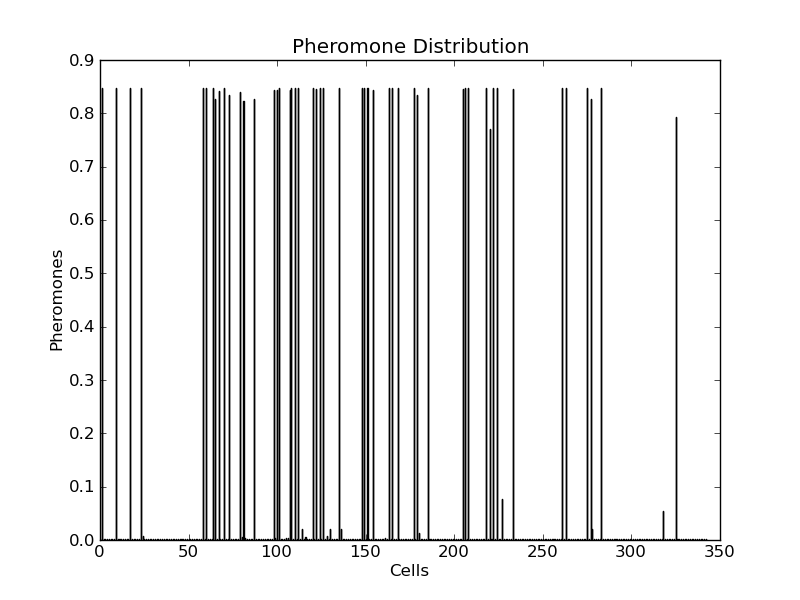
\includegraphics[scale=0.35]{pictures/no_propagation_graph}
		\caption{Pheromone distribution without pheromone propagation in the final iteration of the optimization of a Morse cluster with 50 atoms.}
		\label{fig:no_propagation_graph}
		\end{minipage}
		\hspace{0.5cm}
		\begin{minipage}[b]{0.5\linewidth}
		\centering
		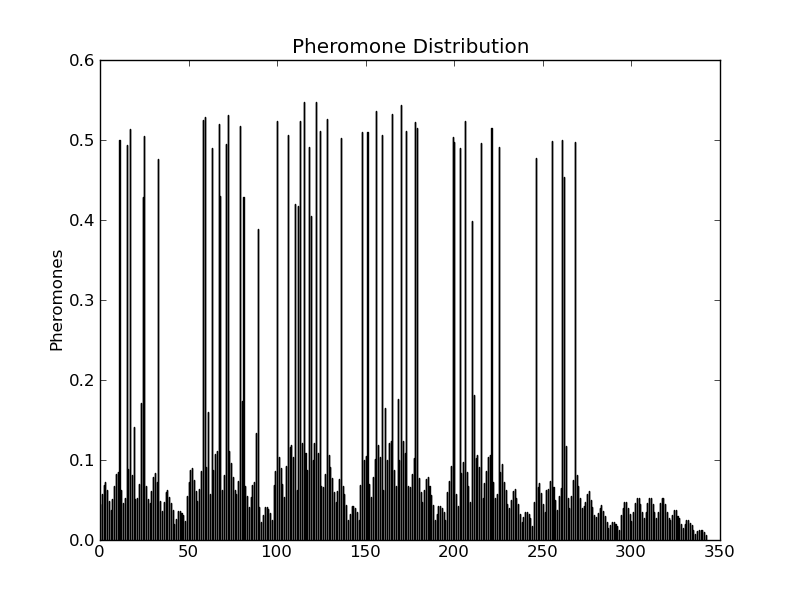
\includegraphics[scale=0.35]{pictures/propagation_graph}
		\caption{Pheromone distribution with pheromone propagation in the final iteration of the optimization of a Morse cluster with 50 atoms.}
		\label{fig:propagation_graph}
		\end{minipage}
		\end{figure}
		
		%\botapic[0.45]{no_propagation_graph}{Pheromone distribution without pheromone propagation in the final iteration of the optimization of a Morse cluster with 50 atoms.}
		%\botapic[0.45]{propagation_graph}{Pheromone distribution with pheromone propagation in the final iteration of the optimization of a Morse cluster with 50 atoms.}	
		\begin{table}[!htdp]
				\begin{center}
					\begin{tabular}{| c | c | c | c | c |}
						\hline
						\textbf{Instance} & \multicolumn{2}{c|}{\textbf{DACCO}} & \multicolumn{2}{p{4cm}|}{\textbf{DACCO without pheromone propagation}} \\ \hline
						~ & SR & MBF & SR & MBF \\ \hline
						30 & 28 / 30 & -106.831095 & 25 / 30 & -106.824054 \\ \hline
						38 & 25 / 30 & -144.053535 & 22 / 30 & -143.893024 \\ \hline
						45 & 3 / 30 & -174.295931 & 2 / 30 & -174.311589 \\ \hline
						50 & 12 / 30 & -197.853115 & 10 / 30 & -197.652445 \\ \hline
					\end{tabular}
					\caption{Optimization results obtained by DACCO with and without Discrete Local Search in the selected Morse cluster instances}
					\label{tab:pheromone_propagation_results}
				\end{center}
		\end{table}
		% \begin{table}[!htdp]
		% 			\begin{center}
		% 				\begin{tabular}{| c | c |}
		% 					\hline
		% 					\textbf{Instance} & \multicolumn{1}{p{4cm}|}{\textbf{DACCO - DACCO without Discrete Local Search}} \\ \hline
		% 					30 & $\sim$ \\ \hline
		% 					38 & $\sim$ \\ \hline
		% 					45 & $\sim$ \\ \hline
		% 					50 & $\sim$ \\ \hline
		% 				\end{tabular}
		% 				\caption{Statistical results of comparing DACCO and DACCO without pheromone propagation}
		% 				\label{tab:statistical_comparison_pheromone_propagation}
		% 			\end{center}
		% 	\end{table}
		
		
	